\documentclass{article}

\usepackage{siunitx} % Provides the \SI{}{} and \si{} command for typesetting SI units

\usepackage{graphicx} % Required for the inclusion of images

\usepackage{tabularx} % Tables

\usepackage{natbib} % Required to change bibliography style to APA

\usepackage{amsmath} % Required for some math elements

\usepackage[letterpaper,top=2cm,bottom=2cm,left=3cm,right=3cm,marginparwidth=1.75cm]{geometry}

% Many options for pseudocode
\usepackage{algorithm2e}
\usepackage{algorithmic}

\usepackage{listings} % Python code blocks

\setlength\parindent{0pt} % Removes all indentation from paragraphs

\title{Lab 3 Report: Wall Following on the Racecar} % Title

\author{Team 10 \\\\ Jeremiah Budiman \\ Miranda Cai \\ Tiasa Kim (Editor)\\ Bill Kuhl \\ Savva Morozov \\\\ MIT 6.141/16.405 \\ Robotics: Science \& Systems\\} % Team # + Names, Class (RSS)

\date{March 4, 2022} % Date for the report

\begin{document}
\maketitle
\section{Introduction}
\author{Tiasa Kim}

\subsection{Objective}
Building on from the previous lab where we implemented an autonomous wall following controller in simulation, Lab 3 introduces a more comprehensive approach to autonomous systems by introducing physical hardware, including a mini racecar, LIDAR sensor, ZED camera, IMU, TX2 compute board, motor battery, router, and two power cables. \\

The main objective(s) of the lab was to: 
\begin{itemize}
    \item gain familiarity with the racecar environment and hardware setup
    \item implement a functional wall-following code to get the physical racecar to autonomously drive forward while maintaining a desired distance from the detected wall
    \item implement a safety controller to prevent the car from collision and inflicting costly damage
\end{itemize}

\subsection{Overview}
Implementing a working wall follower allows for a more complex and integrated autonomous system as we will tackle topics of object detection, perception, and planning in future labs. Likewise, the controller built in this lab has important practical applications since real-world deployment of autonomous vehicles requires a reliable control system for close lane detection and maintenance to prevent traffic collisions. Furthermore, building a dependable safety mechanism is essential for the financial reasons being that the racecar and supportive hardware are very expensive resources, but also for the greater societal importance of protecting drivers and pedestrians from accidents and fatalities. The work in this lab, thus, can be understood as the building block for a robust and scalable autonomous system where reliable safety and accuracy are essential components. \\

With these objectives in mind, we designed and implemented an autonomous controller system using a 2-step solution approach where the first step is to implement a line-detecting mechanism using least-squares regression and a low-pass filter to reduce extraneous data points. The following step is to apply a pure-pursuit controller method where the level of aggression in the controller is dependent on the margin of error with respect to the desired trajectory. \\

\section{Technical Approach}
\author{Tiasa Kim}
\subsection{Technical Problem}
Given the inputs of a point cloud of laser scan messages detected by the LIDAR and a desired distance (cm) at which the car should maintain from an arbitrary wall on the left or right side, the output produced by the system is an Ackermann Drive command indicating a steering angle and velocity at which the racecar should drive to maintain its desired distance. With the known inputs and expected form of output, the lab challenge was to process the LIDAR (laser scan) data using ROS publisher / subscriber nodes and topics and implement two autonomous controllers - a wall follower and a crash-prevention safety controller. \\

Because events in the real world are rather unpredictable, it is important that the control system is robust enough to handle various test scenarios including both low and high speeds, sharp turns, narrow lanes, and multiple forms of obstacles. Thus, the key criteria for the controllers entails enabling the racecar to consistently travel against a detected wall (on which side is dynamically chosen) from its desired distance and in conjunction respond quickly to high- and low-risk situations. 

\subsection{Initial Setup}
Our initial approach to tackling the lab challenge as a team was to first discuss our individual strategies in the previous lab. By outlining what worked and didn’t work, we were able to identify key techniques that could be useful in our consolidated code. The process of deciding which techniques exactly to incorporate involved a qualitative and quantitative assessment based on verbal reporting on individual test scores and observed effectiveness. Our integrated approach correspondingly followed point-cloud filtering using a low-pass filter, least-squares fit for line-finding, an offset function to find the desired vehicle trajectory, and a pure-pursuit controller. \\

\author{Miranda Cai}
\subsection{Technical Solution (Wall Detection)}
\subsubsection{Point Cloud Filtering}
The first step in order to accurately detect the wall was to parse the distance readings of objects taken by the LIDAR and save only the relevant information. Specifically, since the goal of this lab was simply to follow a wall either on the left or the right side of the racecar, we only needed to process data for the corresponding side. To do so, we started off by saving the points within a specified angle range depending on the side of the wall. We found through trial and error that incorporating either too many readings behind the racecar or not enough in front made the car detect corners too slowly and crash into the new wall. On the other hand, incorporating too many points caused the car to initiate its turns too quickly and fall off the desired distance. In the end, we found that collecting angles (degrees) within the range [-25, 90] for left-sided walls and [-90, 25] for right-sided walls with respect to the front of the racecar worked well.\\

To minimize the amount of noise in our data, we added a second layer of filtering to our points prior to simulating the wall. We removed all points greater than a threshold distance from the racecar, which was calculated by multiplying the desired distance to the wall by a constant. For example, in a narrow hallway, it was likely that any reading greater than three times our desired distance would add unwanted noise when we tried to map the wall, hence we removed these points as part of our pre-processing. As a general case, to account for the possibility that the racecar could start in an open area far away from any wall, if no readings are within the threshold value, we would gradually increase our constant multiplier until a minimum number of points become valid. 

\subsubsection{Least Squares Regression}
After cleaning up our readings, we used a least-squares regression model to create a line that best fit our wall. Because the LIDAR readings were given in the form of a LaserScan which contained both information on the angle of a point and its corresponding distance with respect to the front of the racecar, we were able to calculate the 2D coordinates of each point with the racecar as the origin (0,0). From here, we fed the coordinates into a least-squares model, and found the line of best fit by generating the line’s slope and y-intercept. This line represented the location and orientation of the wall in the car’s coordinate system. Since this line would eventually be used as an input into our pure-pursuit trajectory algorithm explained in the Section 2.4, we offset the y-intercept by the desired distance, making the line represent the racecar’s desired trajectory instead.

\subsubsection{Low-Pass Filtering}
As a final attempt to minimize noise, we implemented a low-pass filter on the slope of our line. In short, we set the current line’s slope by taking a weighted average of the previous line’s slope and the slope calculated through least-squares. This filter helped to reduce the effect of a line calculated with erroneous readings, such that the racecar’s trajectory would continue smoothly.

\subsection{Technical Solution (Pure Pursuit Trajectory)}
\begin{figure}[h!]
\centering
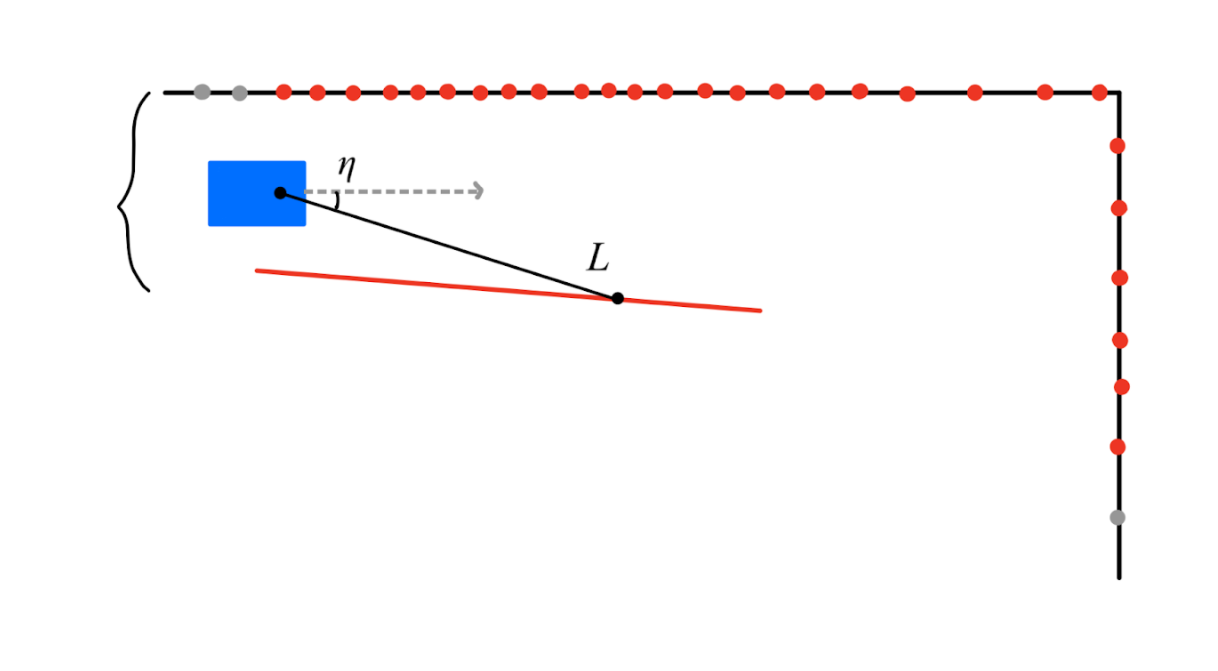
\includegraphics[width=.6\columnwidth]{Screenshot (157).png}
\caption{Choosing and projecting \textit{L}}
\end{figure}
\begin{figure}[h!]
\centering
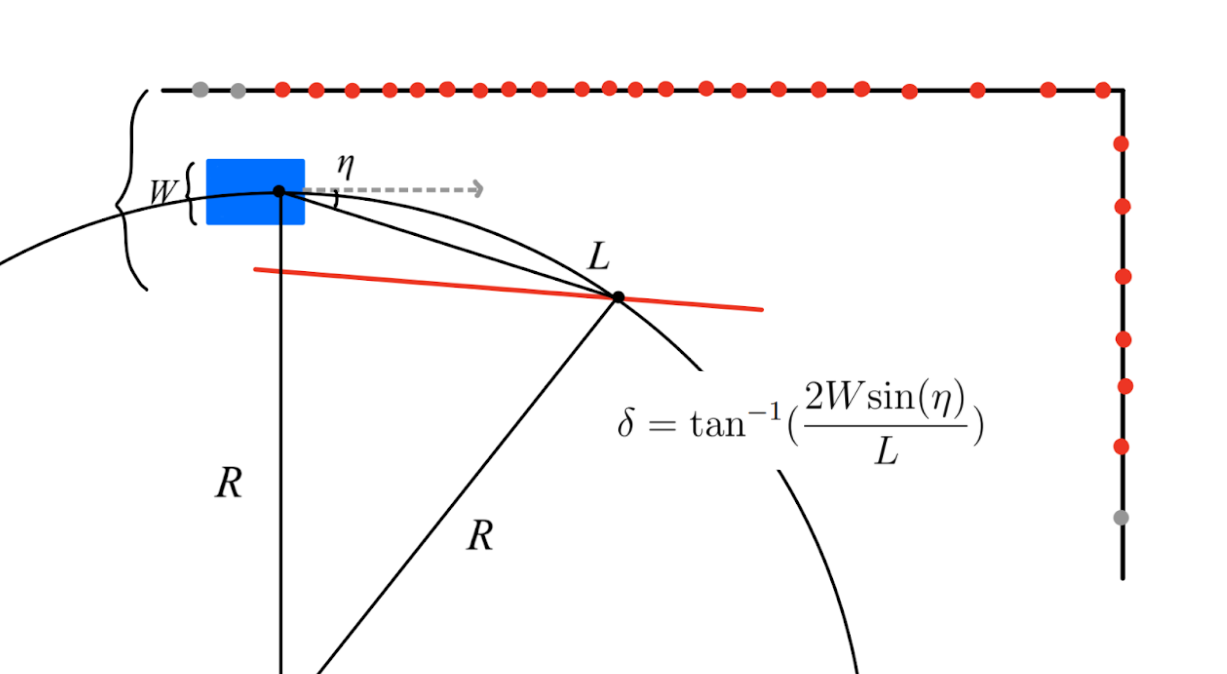
\includegraphics[width=.6\columnwidth]{Screenshot (159).png}
\caption{Calculating path arc and steering angle}
\end{figure}

\subsubsection{How is it implemented?}
In the context of this challenge, pure pursuit is utilized as an algorithm that approximates the path that the racecar will take to reach its desired point as an arc, which we can use to calculate the necessary steering angle output of the racecar. As illustrated in Figure (1), there is a line segment of length \textit{L} connecting our car to the desired trajectory calculated in Section 2.3.2 shown in red. Our first step in pure pursuit is to choose what length we wish \textit{L} to be, and then project \textit{L} onto our desired trajectory to find the point of intersection. Figure (2) demonstrates that an arc representing the racecar’s path is formed by finding the circle that is both tangent to our car and intersecting the projection of \textit{L}. Because a longer \textit{L} directly corresponds to a wider and flatter curvature of the arc, we adjust the length of \textit{L} depending on the racecar’s proximity to the desired trajectory. Specifically, we included the heuristic that if the racecar is greater than a certain threshold distance away from the desired trajectory, we use a larger \textit{L} such that a more conservative approach is taken with our steering to avoid potential oscillations in the future. Otherwise, if we are close enough to our desired trajectory, we can make sharper, shorter turns and reach the desired trajectory almost immediately without overturning.\\

After choosing \textit{L}, we calculate the coordinates of its intersection to the desired trajectory. Using geometry, we were able to find the radius \textit{R} of the circle described previously and drawn in Figure (2). Let \textit{W} be the width of the racecar and $\eta$ be the angle from \textit{L} to the racecar. Then, using \textit{L, R, W, $\eta$}, we can plug these values into the formula below to find the steering angle (radians), $\delta$, to be sent to the racecar as an Ackermann Drive command to follow the path to reach the desired trajectory:
\[\delta=\tan^{-1}({2W\sin(\eta)\over L})\]
Note: This equation is a given in the pure pursuit algorithm.

\subsubsection{Why did we choose it?}
Our team decided to implement pure pursuit over other control systems mainly because of how formulaic and intuitive it is. Pure pursuit requires that we predict the future trajectory of the car, and from there use a series of mathematically sound steps in order to calculate the change in angle needed to reach this trajectory. In comparison, the other option was to use a PID controller, which requires hacking at constants in order to pass specific test cases at a time rather than functioning for the general. In addition, PID controllers for this challenge have a less intuitive conversion from error to process. The necessary process for the car to move closer to or further away from the wall is the steering angle. However, our error is read in terms of distance. While pure pursuit safely converts from distance to angle using geometry, PID ignores the fact that the two terms use different units and bases its conversion off correlation entirely.

\subsection{Crash Safety Control}
\begin{figure}[h!]
\centering
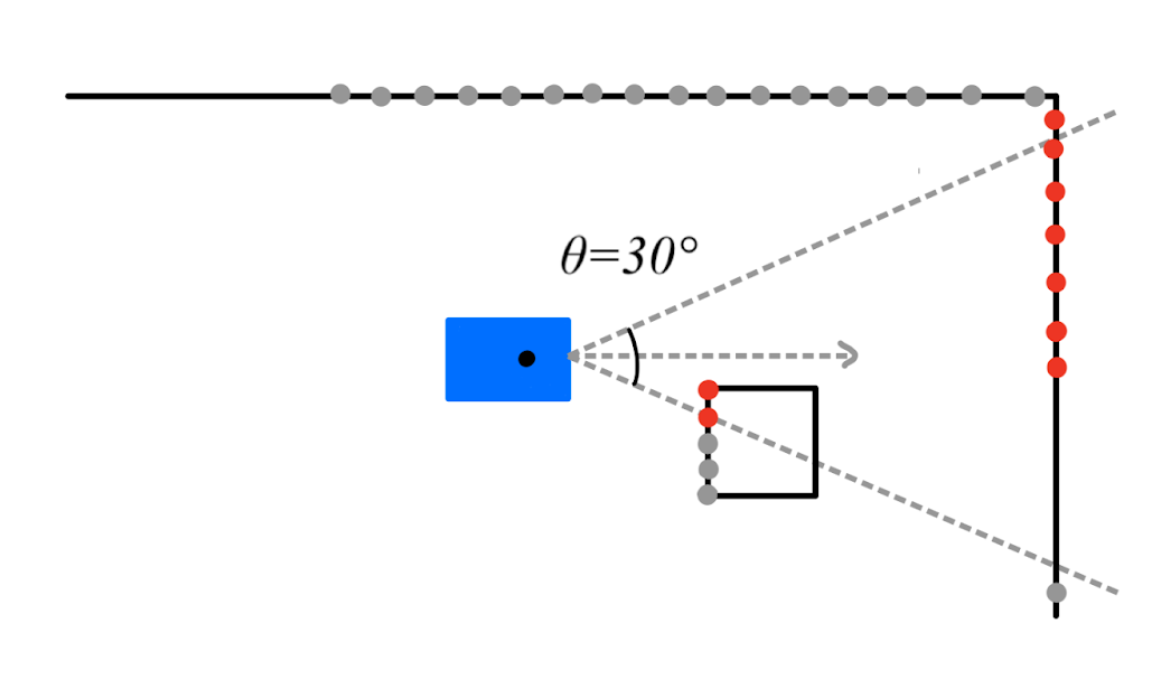
\includegraphics[width=.7\columnwidth]{Screenshot (161).png}
\caption{Racecar detection of potential collision}
\end{figure}
To prevent collision damage, we implemented a safety control on the racecar that completely stops the racecar in the event that it detects an object within a threshold distance from it. Using the LIDAR readings once more, we sort through the distances to the front of the racecar to find the point closest to it. If this minimum distance is within the threshold distance, then we have detected an upcoming collision and set the velocity of the car to 0, bringing the racecar to a halt. While it is important to minimize any risks to the racecar, we also did not want to sacrifice the functionality of the wall follower. Thus, to prevent the car from recognizing the wall we wish to be following as an obstacle, we only check for the minimum distance within a filtered set of distances that all fall between the angle range of [-15, 15] with respect to the front of the car. In doing so, we only search for obstacles directly ahead of the racecar and those that could lie in its current trajectory, as shown in Figure (3).

\section{Experimental Evaluation}
\subsection{Qualitative Analysis}
\author{Jeremiah Budiman} \\

To assess the performance of the robot’s wall following and safety measures, a number of experiments under different parameters and environments were carried out. Qualitatively, it was evident that the car had more stable wall following at lower speeds.

\subsubsection{Test Series 1: Slow Speed – Classroom Track}

First, it was vital the robot could execute simple tasks at slow speeds. These tasks included following a solid straight wall, turning properly at 90-degree corners, and stopping before colliding with an object in front. To test this out, the robot was placed in a small-to-medium-sized classroom that included four 90-degree corners. The robot was set to a conservative speed of 1~\si{\meter\per\second} and a desired distance of 50 cm from the wall. A white canister was also placed at the end of the course to test for the robot’s safety controller. While the car was running the course, a rosbag recording was taken, capturing points detected by the LIDAR and showing the target trajectory based off the detected wall. \\

The robot successfully executed these tasks with the given parameters. As shown by Figure 4 from the rosbag recording in the upper right corner, the target trajectory (depicted by the bold red line) is parallel and follows the real wall (outlined by the LIDAR points) fairly well, displaying successful wall following. \\

\centerline{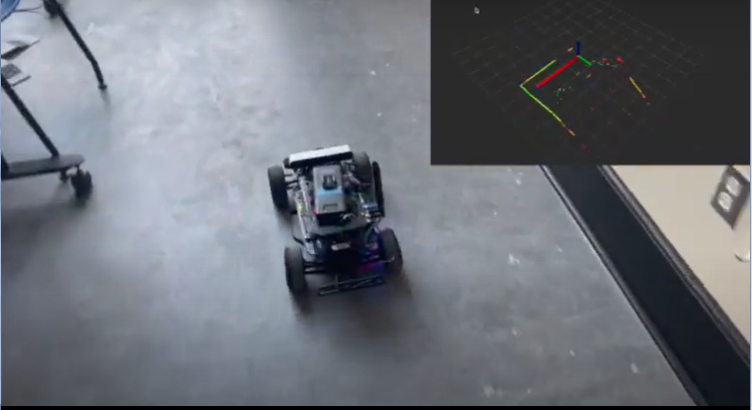
\includegraphics[width=.5\columnwidth]{pic1.png}}

\begin{center} 
    Figure 4: Projected path parallel to detected wall 
\end{center}

	Notably, the car demonstrated smooth cornering ability. In general, it is common for car that is not robustly designed to do one of two things when turning at corners of sharp degree. First, the car might not turn sharp enough, resulting in the car coming too close to the wall when executing the turn. Second, the car may overshoot the turn and swing past the turn, resulting in the car having to turn slightly in the opposite direction after completing the course to adjust for the overshoot. As a positive outcome, our racecar exhibited none of these behaviors during this test. As shown in Figure 5, even before the robot completed its turn, the desired trajectory shown in the rosbag recording is parallel to the new wall detected, preventing an overshoot of a turn. \\
	
	\centerline{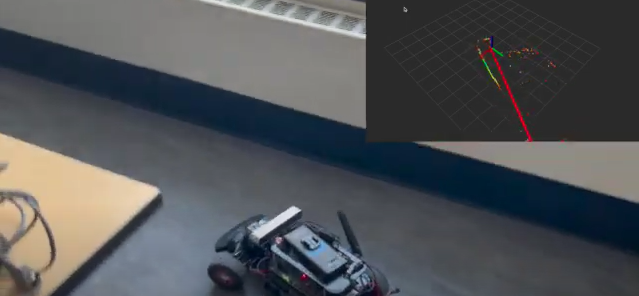
\includegraphics[width=.5\columnwidth]{pic2.png}}

\begin{center} 
    Figure 5: Smooth cornering around sharp turns 
\end{center}
	
	Lastly, the car terminated before hitting the white canister at the end of the course. Overall, the test signifies the robot's robustness under slow speeds. Two tests were completed with the given parameters. Both replicated accurate wall following behaviors. \\
	
\subsubsection{Test Series 2: High Speed – Corridor Track }

The second series of tests included putting the robot in a long hallway corridor at high speeds (2~\si{\meter\per\second}) with a desired distance of 70 cm from the wall. It should be noted that the walls in this environment are not constant throughout. Small gaps in the walls were present due to the presence of doors. \\

Qualitatively, these tests failed when assessing the robot’s wall following. Major oscillations were detected in the movement of the physical car, as shown in the rosbag recordings and by the red line (in Figure 6) indicating an nonparallel predicted trajectory to the detected wall from the LIDAR points. This pattern was constant throughout the tests, resulting in high instability when driving. \\

\centerline{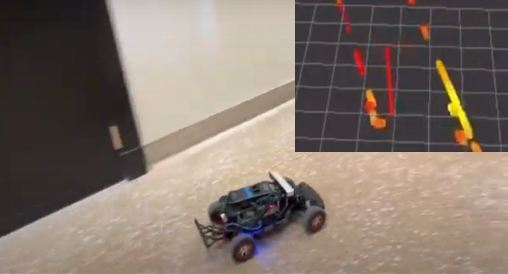
\includegraphics[width=.5\columnwidth]{pic3.png}}

\begin{center} 
    Figure 6: Oscillations in Projected Path 
\end{center}

Four tests were executed in theis series; three resulted in major oscillations but reached the end of the corridor roughly 30 meters away. One test also included major oscillations and resulted in an eventual crash 10 meters from the starting point. \\

Evidently, higher speeds pose a number of issues for the robot. A deeper analysis of both the successful and unsuccessful runs will be explained in the next section.


\subsection{Quantitative Analysis}
\author{Bill Kuhl} \\

After we conducted our physical tests, we analyzed a selection of rosbag files to analyze the performance of our wall follower. These consisted of two types of experiments. The tests labelled "Around the Room" were evaluating the performance of the robot following the wall of a classroom, including turn handling and collision avoidance. The tests labelled "Fast Corridor" were evaluating the speed of the robot following a straight wall in a hallway at higher speeds.\\

Our analysis was conducted in two parts. The first was analyzing the LIDAR maps outputted by the rosbag files overlaid with markers representing the desired path to the target distance from the wall. This proceeded with a quantitative analysis of the algorithm's performance using a similar formula to the one used in class for continuity.\\

Our qualitative analysis method is based on a visual examination of the rosbag / LIDAR visualizations and video of the tests. The tests that were considered successful show the racecar following the wall in a stable manner and are labelled as "Stable Wall Follower". In all other cases, the results are documented describing the discrepancy accordingly.\\

Our quantitative analysis method was designed to elicit a similar metric to the one used in the previous simulation lab to generate comparable results. Due to the obfuscated nature of the grading code, this metric does not compare one-to one to the test files. To calculate our Path Accuracy metric, a script was run for the test portion of our rosbag files, which takes each published LIDAR dataset, measures the distance from the car to the wall, and calculates the error compared to the desired distance. This error is then added to a list that continually grows until the end of the test. Throughout the test, the list is averaged and printed to the terminal to provide a picture of the algorithm's performance. The numbers reported in the Path Accuracy section are reflectively the outputs of the test script at the time of terminating the test.\\

\begin{table}[htbp]
    \centering
    \title{}
    \begin{tabularx}{\textwidth}{| X | X | X | X |}
        \hline
        Test Name & Speed [m/s] & Qualitative Result & Path Accuracy \\ \hline
        Around the Room 1 & 1 & Stable Wall Follower & .87 \\ 
        Around the Room 2 & 1 & Stable Wall Follower & .90 \\ 
        Fast Corridor 1 & 2 & Rapid Oscillations & .65 \\ 
        Fast Corridor 2 & 2 & Rapid Oscillations & .67 \\ 
        Fast Corridor 3 & 2 & Crash & - \\ 
        Fast Corridor 4 & 2 & Unstable Oscillations & .72 \\ \hline
    \end{tabularx}
    \caption{A selection of rosbag files from experiments}
\end{table}

Predictably, the slower tests performed better, averaging .87 and .90 accuracy results respectively. This is more impressive considering it included turning multiple times. This test was run twice to validate its success. The other tests performed with greater error, with accuracy results of .65, .67, and .72 respectively, and one test failing altogether. One of the faster tests failed completely. We ran this test four times compared to the two for the room test to try and isolate the cause of the error. The cause of error will be explained more in the Conclusion section.


\section{Conclusion and Future Steps}
\author{Savva Morozov} \\

In this lab, we successfully adapted and validated our pure-pursuit controller for execution on a hardware platform.
We also implemented and tested a simple safety controller to prevent the car from crashing into the wall.
We observed promising performance at relatively low speeds of 1~\si{\meter\per\second} in environments that lacked reflective surfaces or thin objects.
Conducting additional experiments under more challenging conditions (higher speeds, cluttered environments, corridors) allowed us to determine unforeseen vulnerabilities of our solution:

\begin{itemize}
  \item Going through the corridor, the car exhibited unstable oscillatory tracking behavior due to perturbations in the desired trajectory. 
  These perturbations resulted from poor wall estimation, caused by using erroneous points in the least-squares linear fit.
  We mitigated this problem by limiting the range of points used to estimate the wall, yet we could not test this correction due to our next issue.
  \item Our most recent tests suffered from 10-15 second delays in LIDAR point cloud processing.
  We do not know the cause of this issue, but we expect to resolve it during office hours.
  \item Though sufficient at low speeds, our simple safety controller failed to prevent the car from hitting the wall when running at 2~\si{\meter\per\second}.
  This illustrates that the safety controller must be a function of the car's speed.
  In the future, we will either use multiple heuristic distance-speed cutoffs (instead of just one) or incorporate the vehicle's dynamics in safety assessment.
  \item After resolving the above issues, we intend to fine-tune the controller parameters to empirically find the values that provide the most aggressive yet safest performance. 
  Since we expect to use the same pure-pursuit controller in the next lab, we will address all these issues in the next few days.
\end{itemize}


Finally, we wanted to reflect on our overall technical approach.
Though it has been engaging to see the car perform very nontrivial tasks with only a few lines of code and a simple controller, we had a nagging feeling of disappointment in the capabilities of our code.
The controller was not very generalizable and only performed well under strict assumptions; even slight deviations from these assumptions revealed vulnerabilities in the control policy.
Many such vulnerabilities could be fixed by incorporating additional heuristics into the policy, but doing so inevitably increased the number of tuned parameters.
It did not feel like we were making educated engineering decisions---instead, we were ``hacking" to achieve better performance.
We did see that task-specific heuristic control policies can be very powerful, and per Prof.\ Carlone's advice, we will fully explore the capabilities of such controllers.
Still, we want to learn about more general design solutions in the future.

In particular, we are curious to invest our efforts into richer environment representations and long-horizon planning policies.
Occupancy maps may prove to be useful when racing across the basement of STATA, clearly indicating obstacles in our path.
As for trajectory planning, sampling-based or optimization-based policies are both generalizable and advantageous in the long run.
Such policies could positively impact our performance by considering long-horizon task completion and safety of the robot.
We will keep these ideas in mind as we approach the final stages of the racing competition.





% Summarizes what you have achieved in this design phase, and notes any work that has yet to be done to complete this phase successfully, before moving on to the next. May make a nod to the next design phase.\\\\
% (no more than 500 words)

\section{Lessons Learned}
\author{\textbf{Jeremiah Budiman}} \\

From a CI perspective, I've realized the importance of truly needing to practice presentations before actually presenting. The dry-run exposed me to things I should probably cut out or add in the presentation. It also became apparent what things were clear and not clear based off the feedback from my peers. Additionally, I learned that not meeting in person every time is completely sufficient and not at all a disadvantage. Often times for this lab, people had scheduling conflicts. However, either with zoom or even just through text, we would still be able to communicate properly and pass on ideas. \\

From a technical standpoint, I got to experience first-hand that often times the real-world test does not match with the simulation. I also learned that often times, it is the easiest solution that fixes the issue, not the hardest. For example, when creating the safety controller, we simplified the solution even further and only then did it work properly. \\

From a collaboration standpoint, I got to learn more about my teammates and what they're strengths were. Overall, I am very happy with our team dynamic and believe there's a diverse group of talent with everyone willing to help each other. \\

\author{\textbf{Miranda Cai}} \\

In terms of the CI part of this class, I've realized that it's a lot harder to work on the same robot with others than I originally thought. While I try to be as involved as possible, a lot of the time we each get caught up in the individual work that we're doing and forget to communicate our progress. At this point, it takes a while to regroup, and I've learned that a better way to divide and conquer would be to have more periodic check-ins and a clear division of parts before we each start doing what we want.\\

As for the technical lessons, I've learned so many new concepts such as pure pursuit, low-pass filtering, and different heuristics to make my strategies more complex. This was my first time working with a real robot, and it was interesting to see how things differed when implemented on the simulator vs in real life (i.e. velocities that worked in the simulator failed in real life). I'm really grateful to my teammates for guiding me and teaching me new ways to approach problems.\\

\author{\textbf{Tiasa Kim}} \\

If there is one key takeaway or lesson learned from this lab, it is that the end result or deliverable is not all that matters. Although yes, our team may have implemented a working wall follower and safety controller, put together and delivered a rather successful presentation, and submitted our deliverables on time, a lot of what was regretfully missing in the internal makings was the communication and collective team support. What I wished we (or perhaps I) had done was opened up the space to have an honest discussion on team dynamics and set up better-defined expectations on roles that utilize - rather than dampen - our individual strengths. I am a strong believer that each one of us is capable of contributing meaningful work, but so often recognizing one’s actual contributions is lost when we act without listening or trying to understand others. Moving forward, I hope to balance out team dynamics so that no single person is ever dominating the conversation (with their literal words or ideas). Furthermore, I wish to work on being a more solution-led teammate and leader by better navigating lack of communication and unresolved conflicts. By the end of this semester, I hope I can attest to the growth and mutual bond in our team - not just the success in technical aspects of the class learning objectives. \\

Aside from team dynamics, a technical lesson I gained is that pure-pursuit can be a more effective controller (as compared to PID controller) and can be implemented by defining (via heuristic evaluation) a distance $L$ from the car’s current position and a point on the line trajected by the DESIRED$\_$DISTANCE parameter and a radius $R$ determined by the line tangent to the point representing the car’s current position and the point intersecting the line $L$. Additionally, this method can be combined with a point-cloud filtering technique like a low-pass filter to reduce extraneous or “noisy” data points that might skew the accuracy in detecting the line/wall.\\

\author{\textbf{Bill Kuhl}} \\

From a communication perspective, this lab was challenging in it's technical simplicity. Because much of the work was already written and created, we were working in a group of 5 trying to accomplish tasks that could only be done on one computer. An immediate challenge was that we could not all meet at the same time. I ended up being the only one who couldn't make the meeting time, which ended up working OK, because I was able to contribute asynchronously before the meeting. Additionally, it can be challenging to have 4 people try and analyze and tune the same 2 parameters. In the future when there is more work I believe this particular challenge will be negated due to necessity. For writing up the reports and presentations, we did a good job of parallelizing the work. I worked with Jeremiah on the Experimental Evaluation section, and within that we broke it up again so that we could work asynchronously. This was highly effective, and we were able to complete our work without headache.\\

From a technical perspective, I learned the importance of writing well-documented and transferable code. Because I had to work asynchronously, I had to make sure that everyone on the team understood the safety controller I wrote and could integrate it into the other code. Additionally, when I was writing scripts to analyze the bag files, there were some published ROS topics that were created by the rest of the team which I needed to understand to correctly analyze the script and data.\\


\author{\textbf{Savva Morozov}} \\

Effective communication with each other was the biggest challenge we faced.
As we worked on the technical components of the lab, we did not delegate specific tasks well.
This was largely because the lab is inherently linear and can be completed by one person in a span of a few hours, as the lab builds upon the work we've already done.
Yes, I think this lab was designed poorly — it is not a team-based lab.
I am not trying to shift the blame — I fully acknowledge that we could have set up our expectations from each other more precisely instead of awkwardly brushing the details under the rug.
I believe we are already working in the right direction with lab 4, having delegated individual components to each other; I will also be sure to solidify our timeline with the team later today.
Judging by these reflections, my teammates are on the same page with me---improving communication is our main focus. \\

Reflecting on the CI component of the class, I have to say that I did not expect to get a B- for the presentation we gave. 
I have done B- work in the past, and this did not feel like it. 
I underestimated what was expected from us, so I will be putting more effort into the CI component of the class. \\

As for the technical difficulties, I certainly had issues and frustrations during this lab---troubleshooting network connectivity, debugging the code, parameter tuning, etc. 
However, having worked with drones and walking robots in the past, I fully expected to have such problems, so they do not bother me as much.
I did spend quite a few hours solving these issues---hopefully, this won't be as much of a case with the future labs, as we would be able to delegate technical responsibilities more effectively.
\end{document}
